\documentclass[letterpaper]{article} % DO NOT CHANGE THIS
\usepackage{aaai2027}  % DO NOT CHANGE THIS
\usepackage[hyphens]{url}  % DO NOT CHANGE THIS
\usepackage{graphicx} % DO NOT CHANGE THIS
\urlstyle{rm} % DO NOT CHANGE THIS
\def\UrlFont{\rm}  % DO NOT CHANGE THIS
\usepackage{natbib}  % DO NOT CHANGE THIS AND DO NOT ADD ANY OPTIONS TO IT
\usepackage{caption} % DO NOT CHANGE THIS AND DO NOT ADD ANY OPTIONS TO IT
\frenchspacing  % DO NOT CHANGE THIS
\usepackage{booktabs}
\usepackage{amsmath}
\usepackage{amssymb}
\usepackage{tikz}
\usetikzlibrary{positioning,arrows.meta,decorations.pathreplacing}
\pdfinfo{
/TemplateVersion (2027.2)
}
\setcounter{secnumdepth}{1}

\newcommand{\code}[1]{\texttt{#1}}
\newtheorem{theorem}{Theorem}
\newtheorem{definition}{Definition}

\title{When the Shield Is Not the Actuator: Machine-Checked Revocation Bounds\\for AI Controllers of Stock Motor Drives}
\author{
    Utkarsh Maurya
}
\affiliations{
    VolnLabs\\
    utkarsh@volnlabs.com
}

\begin{document}

\maketitle

\begin{abstract}
AI controllers, from learned policies to language-model planners, increasingly command physical
actuators, and runtime assurance assumes they can be revoked: a monitor, an operator or a
Simplex switch hands control to someone else. Industrial actuators make revocation harder than
it looks. A motor drive keeps executing the last setpoint it accepted, and buses can hold frames
for arbitrarily long, so the revoked controller's command can keep acting after the switch. Worse,
an energy interlock held by the \emph{new} authority will happily power the \emph{old} one's
command. We call this a setpoint hijack. We give a protocol, enforced by a small trusted gate in
front of an unmodified drive, and a machine-checked bound: from $t_c + W + T + \delta$ on, where
$t_c$ is the revocation, $W$ a challenge window, $T$ a lease and $\delta$ the output's shutdown
delay, an energized output takes from the revoked controller neither its energy, nor its
committed setpoint, and every pending frame of that controller is fenced off from the drive. The
bound holds in a Lean model with unbounded bus delay, a finite id space, gate resets, and a gate
that never hears of the revocation, and scales with the gate's clock rate under drift. On the
gate's C firmware we prove the timing rules for unbounded runs with CBMC, and check the full
property, including the drive side, by small-scope exhaustive exploration and by
software-in-the-loop tests against the unmodified CAN code of an open-source drive (ODrive).
These checks and an independent review found nine bugs in our own artifacts, most where a layer
above abstracts. All evidence is software; $\delta$ and the motor are left to hardware work.
\end{abstract}

\section{Introduction}

AI systems now close the loop on physical machines. Vision-language-action models emit robot
actions \citep{brohan2023rt2}, language models sequence skills on real
robots \citep{ahn2022saycan}, and learned policies drive manipulators and vehicles. None of these
is verified end to end \citep{seshia2022verifiedai}, so deployments rest on runtime assurance: a
shield filters unsafe actions \citep{alshiekh2018shield}, a Simplex switch hands control from an
advanced controller to a verified safe one \citep{sha2001simplex,phan2020nsa}, or a human
interrupts the agent \citep{orseau2016interruptible,hadfield2017offswitch}. All of these treat the
switch as the end of the agent's influence. Once control is handed over, the agent's actions no
longer reach the plant.

On a factory floor this is false in a specific way. The agent's commands reach a motor through a
fieldbus and a drive. A drive keeps executing the last setpoint it accepted, because that is what
makes it a drive. Frames can sit in transmit mailboxes, bus queues and receive buffers for
arbitrarily long. Revoking a controller therefore does not stop its last command: the command
keeps acting until something overwrites or de-energizes it. The obvious remedy is an energy
interlock, like Safe Torque Off \citep{iec61800}, driven by a lease: energy only while the current
authority holds a live lease. That remedy has a hole. If the old controller's frame arrives after
the new controller's lease has enabled energy, the drive runs the old controller's command, under
the new controller's power. We call this a \emph{setpoint hijack}, and show it reachable in proof
when the gate controls energy alone, and show on the drive's real code that the late command is
installed (Section~\ref{sec:hijack}).

The question this paper answers is: \emph{after an AI controller is revoked at time $t_c$, by when
is the physical output provably free of it, if the drive is stock and untrusted?} Our answer is a
protocol enforced by a small trusted gate in front of the drive, and a bound of
$t_c + W + T + \delta$ that is machine-checked under adversarial timing. The gate need not
understand or trust the AI controller, the bus or the drive. It needs only to own the drive's
command and energy paths.

\paragraph{Contributions.}
\begin{itemize}
\item \textbf{The hazard, proved.} A gate that controls energy alone admits a setpoint hijack. With
hidden commits and unbounded delay, no gate policy that only observes can be both safe and live
across a controller change once a frame may have been lost, so some fence on the drive's side is
necessary.
\item \textbf{A protocol and a composed timed theorem} in Lean~4 \citep{demoura2021lean4}: after
$t_c + W + T + \delta$, an energized output takes neither energy nor its committed setpoint from
the revoked controller, and the controller's pending frames are fenced, under unbounded delay,
finite ids and gate resets, with a gate that is never told of the revocation, and with a deadline
scaled by the clock rate under drift. Each rule in Table~\ref{tab:rules} has a mechanised
counterexample when dropped, in the full model or one of its components.
\item \textbf{A retrofit for a stock drive.} The ODrive v3 firmware's CAN node-id check becomes
the fence, and a free field of its setpoint frame becomes a session tag for readback. Both are
checked in software-in-the-loop (SIL) on the drive's unmodified CAN code.
\item \textbf{Evidence that reaches the firmware.} The gate's timing rules are proved on its C code
with an inductive CBMC harness \citep{clarke2004cbmc}; the code is also explored exhaustively,
at small bounds, against the full finality property, tested
in SIL, mutation-checked, and run as an STM32F4 image in emulation. We report the nine bugs these
checks and review found in our own artifacts, and what found each.
\end{itemize}

All evidence is software. We have not run the gate on a motor; the shutdown delay $\delta$ is an
assumption, and we say where it enters.

\section{System Model and Problem}
\label{sec:model}

\begin{figure}[t]
\centering
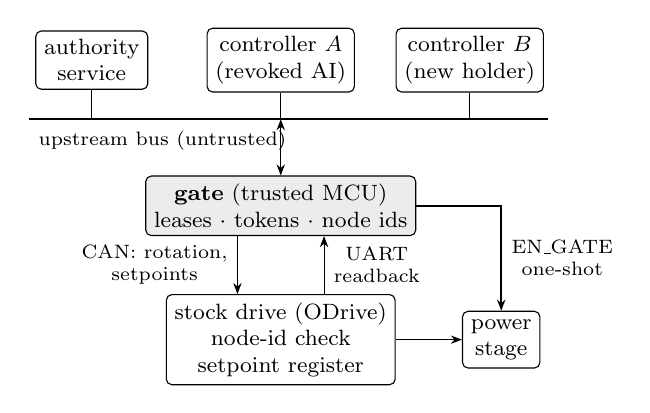
\begin{tikzpicture}[
  box/.style={draw, rounded corners=2pt, align=center, font=\footnotesize, inner sep=3pt},
  lab/.style={font=\scriptsize, align=center},
  >={Stealth[length=4pt]}]
\node[box] (auth) at (0,0) {authority\\service};
\node[box] (a) at (2.4,0) {controller $A$\\(revoked AI)};
\node[box] (b) at (4.8,0) {controller $B$\\(new holder)};
\draw[thick] (-0.8,-0.75) -- (5.8,-0.75);
\node[lab, anchor=north west] at (-0.8,-0.78) {upstream bus (untrusted)};
\foreach \n in {auth,a,b} \draw (\n.south) -- (\n.south |- 0,-0.75);
\node[box, fill=gray!15] (gate) at (2.4,-1.85) {\textbf{gate} (trusted MCU)\\leases $\cdot$ tokens $\cdot$ node ids};
\draw[<->] (2.4,-0.75) -- (gate.north);
\node[box] (drive) at (2.4,-3.55) {stock drive (ODrive)\\node-id check\\setpoint register};
\node[box] (out) at (5.2,-3.55) {power\\stage};
\draw[->] ([xshift=-0.55cm]gate.south) -- node[lab, left] {CAN: rotation,\\setpoints} ([xshift=-0.55cm]drive.north);
\draw[<-] ([xshift=0.55cm]gate.south) -- node[lab, right] {UART\\readback} ([xshift=0.55cm]drive.north);
\draw[->] (drive.east) -- (out.west);
\draw[->, thick] (gate.east) -| node[lab, pos=0.75, right] {EN\_GATE\\one-shot} (out.north);
\end{tikzpicture}
\caption{System. Controllers, including revoked ones, keep upstream access. The gate is the only
path to the drive's command bus, UART and energy enable (EN\_GATE, driven by a hardware one-shot
timer, Section~\ref{sec:protocol}). The drive and both buses are untrusted and may delay, drop or
reorder frames.}
\label{fig:system}
\end{figure}

Figure~\ref{fig:system} shows the parties. An \emph{authority service} decides which controller
may act; it grants by minting tokens and revokes by refusing to mint. \emph{Controllers} are AI
agents or humans. A revoked controller is not trusted to stop: it keeps full access to the
upstream bus, and may replay or withhold anything it ever received. The \emph{gate} is a small
microcontroller and is the only trusted component on the control path. The trusted base is the
gate, the authority service, the key they share, and the power stage's enable input; a
compromised authority or key voids the bound. Behind the gate, the
\emph{downstream bus} and the \emph{drive} are untrusted in timing: frames may be delayed without
bound, dropped, reordered, or stuck in a mailbox forever, and the gate never learns when the drive
commits a frame. The drive holds the last setpoint it accepted. The \emph{power stage} energizes
the motor only while the gate's enable line is high, and de-energizes within $\delta$ after it
falls.

Two parameters are the gate's to choose: the lease length $T$ and the challenge window $W$. The
gate never needs to be told of a revocation; it may be partitioned from the authority forever.
Time is discrete, in gate clock ticks, and $W$, $T$ and $\delta$ are measured in ticks.

\begin{definition}[Timed finality]
Let controller $r$ be revoked at $t_c$. The system has \emph{timed finality with deadline $D$} if
in every reachable state with time $\ge t_c + D$ and energized output: (i) no lease that supports
the energy belongs to $r$; (ii) the drive's committed setpoint was not authored by $r$; and (iii)
no pending downstream frame authored by $r$ can still be committed by the drive.
\end{definition}

Condition (iii) is what makes the property hard. A frame stuck in a bus controller is invisible to
the gate and may surface at any time. Leases bound (i), and readback can confirm (ii), but neither
says anything about (iii). The definition concerns the controller's commands, not the physical
state they caused: momentum or position reached before $t_c+D$ remain, and are the safety
controller's to handle.

\section{Why an Energy Gate Is Not Enough}
\label{sec:hijack}

\paragraph{Setpoint hijack.} Suppose the gate enables energy whenever the current holder's lease
is live, and forwards only the holder's commands, but does not otherwise constrain the drive.
Controller $A$ sends setpoint $\tau_A$, which the bus delays. $A$ is revoked; $B$ obtains a lease
and sends $\tau_B$; the gate enables energy. Then $A$'s delayed frame arrives and the drive
installs $\tau_A$. The output is energized under $B$'s valid lease and executes $A$'s command.
No delay is even needed: if $B$'s first frame is lost, the drive still holds $\tau_A$ when $B$'s
lease enables energy. In our Lean product model, a path around the gate (\code{command\_bypass}) or a
gate that forwards any origin (\code{no\_filter}) reaches a state past the deadline with
energized output and the revoked grant's setpoint; in the refined model with an explicit
downstream stage, a gate without confirmed readback or without a check of frames in flight
enables one grant while the drive holds, or may still commit, another grant's command
(\code{reordered\_commit}, \code{lost\_command}). On the unmodified ODrive CAN code in SIL, the
drive installs both $A$'s persistent setpoint and $A$'s late frame, which an enable that follows
$B$'s lease would energize. The same configuration can arise on industrial drives if a safety
fieldbus such as PROFIsafe \citep{iec61784} fences the safe-torque-off channel while motion
setpoints travel as ordinary process data.

\paragraph{No observation suffices.} Could the gate simply wait until the old frames are gone?
We model the gate's enable decision as an \emph{arbitrary} function of its whole observation
history, including readback that is more informative than real drives give. Commits and losses
are hidden. Then for every run in which a frame was lost there is a run with identical
observations in which it is still pending (\code{stuck\_twin}); every safe policy must refuse to
energize after any controller change in which a frame was lost (\code{lost\_frame\_blocks}); and
no timeout helps, for any length (\code{no\_timeout\_helps}). A useful single-controller policy
does exist (\code{singleGrant\_safe}, \code{singleGrant\_energizes}), so the impossibility is
specifically about authority changes. This is the lease-without-fencing problem known from
distributed locking \citep{burrows2006chubby,kleppmann2016locking}, specialized to hidden commits
in a physical device. The remedy is the same in spirit: a \emph{fence} that the receiver checks.

\section{The Protocol}
\label{sec:protocol}

The drive is stock, so the fence must use something the drive already checks. ODrive's CAN
protocol addresses every frame to a 6-bit node id, and the firmware drops every frame whose id
differs from its current one before dispatching it. The node id can be changed at run time. The
gate turns this into an epoch fence.

\paragraph{Tokens and leases.} A controller asks the gate for a challenge. The gate sends a
counter value with a 32-bit tag under a key it shares with the authority, so the authority can tell
the gate issued it. The authority mints a token, a message authentication code (MAC) over
(controller, flags, challenge), only for
a controller it currently authorizes and only for a tagged challenge. The gate redeems a token only
for its open challenge and only within $W$ of first sending it; redemption grants a lease of
length $T$. Challenge and session counters survive resets. The session counter is stored as is;
the challenge counter is stored as a reserved ceiling, and a reset resumes above it, which saves
flash writes.

\paragraph{Fence.} Each new holder gets a session with a \emph{fresh} node id, one not used
since the last flush. The gate rotates the drive to it and addresses only the holder's setpoints
to it. A stale frame of the previous holder carries an old id and is dropped by the drive, however
late it arrives. With $K$ ids, at most $K-1$ handovers fit between flushes. A \emph{verified
flush} aborts the gate's transmit mailboxes and resets the drive, and only then frees the ids.
Downstream the gate sends only two commands, the node-id change and the setpoint, so no
controller can reach the drive's configuration. The simplest alternative, a verified flush at
every handover, also meets the bound, but reboots the drive with energy off on each change; the
id pool amortizes it to one flush per $K-1$ handovers.

\paragraph{Session-tagged readback.} Before enabling energy the gate reads back, over a UART link
it owns, that the drive holds the holder's setpoint. Value readback is not enough: a value-equal
stale frame would pass. ODrive prints floats with at most six decimals into a ten-character
buffer, so a tag in the low mantissa bits is invisible. Instead the gate runs the drive in torque
mode with passthrough input and sends every setpoint as \code{SET\_INPUT\_VEL} with the velocity
field set to a session tag (node id $+\,1$) and the torque field set to the value. In this mode
the velocity input is unused by the controller, so the tag is free. The gate checks the tag; the
value travels in the same frame (but see Section~\ref{sec:limits}).

\paragraph{Energy.} EN\_GATE is not a pin level but a hardware one-shot timer, re-armed on every
loop for the time left on the lease. A hung firmware loop cannot keep the output energized past
the lease, and the gate's clock is a free-running hardware counter.

\paragraph{Make-before-break.} A handover from a confirmed holder may keep energy on while both
leases are live, until the new holder's setpoint is read back. Energy on the previous holder's
lease alone is unsafe (Table~\ref{tab:rules}).

\paragraph{Parameters.} Our firmware defaults are $W = 50$\,ms and $T = 200$\,ms, so the revoked
controller's influence ends by $t_c + 250\,\text{ms} + \delta$ (Figure~\ref{fig:timeline}). The
price is traffic: a holder renews by a challenge, a token from the authority and a redemption at
least once per $T$, and a handover costs one rotation and one readback. A shorter $T$ tightens the
bound and raises the renewal rate; $W$ must cover the round trip to the authority.

\begin{figure}[t]
\centering
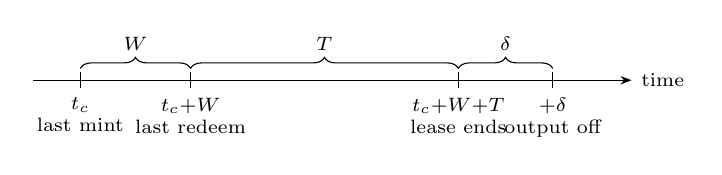
\begin{tikzpicture}[lab/.style={font=\scriptsize, align=center}, >={Stealth[length=4pt]}]
\draw[->] (0,0) -- (7.6,0) node[lab, right] {time};
\foreach \x/\t in {0.6/{$t_c$\\last mint}, 2.0/{$t_c{+}W$\\last redeem}, 5.4/{$t_c{+}W{+}T$\\lease ends}, 6.6/{$+\delta$\\output off}}
  \draw (\x,0.1) -- (\x,-0.1) node[lab, below] {\t};
\draw[decorate, decoration={brace, amplitude=4pt}] (0.6,0.15) -- node[lab, above=3pt] {$W$} (2.0,0.15);
\draw[decorate, decoration={brace, amplitude=4pt}] (2.0,0.15) -- node[lab, above=3pt] {$T$} (5.4,0.15);
\draw[decorate, decoration={brace, amplitude=4pt}] (5.4,0.15) -- node[lab, above=3pt] {$\delta$} (6.6,0.15);
\end{tikzpicture}
\caption{Worst case of the bound. The authority stops minting at $t_c$; a token minted then is
for a challenge sent no later than $t_c$, redeemable for at most $W$ after that, and gives a lease
of $T$. The output follows the enable within $\delta$. The fence and readback remove the revoked
controller's setpoints from that point on, however long its frames stay on the bus.}
\label{fig:timeline}
\end{figure}

\begin{table}[t]
\centering
\footnotesize
\begin{tabular}{@{}p{3.05cm}p{4.3cm}@{}}
\toprule
Rule dropped & Mechanised counterexample \\
\midrule
authority mints only for valid grants & lease renewed after revocation \\
no authority rollback & revoked grant revalidated, renewed \\
challenge window $W$ & pre-revocation token redeemed late \\
energy-path exclusivity & output on with no lease \\
command filter / exclusivity & setpoint hijack \\
fresh node ids & reused id revives a stuck frame \\
verified flush & unverified flush, same \\
session-tag readback (not value only) & value-equal frame hides a lost rotation \\
counters survive reset & old token replayed, or old session tag passes \\
both leases in handover & old holder's energy runs new frame \\
expiry latch (32-bit clock) & ended lease live again after $2^{31}$ ticks \\
\bottomrule
\end{tabular}
\caption{Rule necessity. Each row is a Lean theorem, in the full model or one of its component
models, giving a reachable state that breaks finality, the fence's safety property, or (for the
latch) the deadline test when the rule is removed. Overlap only from a \emph{confirmed} holder
is shown necessary by exploration mutants, not in Lean.}
\label{tab:rules}
\end{table}

\section{Mechanised Results}
\label{sec:lean}

The models are in Lean~4 core with no libraries: seven files, about 3{,}000 lines and 96
theorems, with no \code{sorry} and only Lean's standard axioms. The central model,
\code{FencedFinality}, composes the authority service, tokens with window $W$, leases, a gate
with finite ids, rotation, readback, flush and resets, a downstream stage where frames may be
lost, reordered or stuck forever, a drive that accepts frames only at its current id, and an
output stage that may rise only on the gate's enable and falls within $\delta$ of it going low.
Time advances unconditionally. Notification of the revocation to the gate is a step that may
never happen.

\begin{theorem}[\code{Fenced.finality}]
For every reachable state $s$ with $\delta \ge 1$: if grant $r$ (one controller's authorization;
one revoked grant per run) was revoked at $t_c$,
$s.\mathit{now} \ge t_c + W + T + \delta$ and the output is energized, then the holder's and
the previous holder's supporting leases are not $r$'s, the drive's committed setpoint was not
authored by $r$, and every pending frame authored by $r$ is addressed to an id other than the
drive's current one.
\end{theorem}

The last conjunct is a state property; condition (iii) of the definition follows because ids are
reused only after a verified flush. The proof is an inductive invariant over all steps. The $W$
term is the price of a gate that is
never told: a token minted just before $t_c$ can still be redeemed up to $W$ later. Further
results in the same model:

\begin{itemize}
\item \code{Drift.finality\_real}: if the gate's clock ticks at least once every $R$ units of real
time, the conclusions hold from real time $t_c + R(W + T + \delta + 1)$.
\item \code{recoverable}: with $K \ge 2$ ids and $T > 0$, from any reachable state, including
exhausted ids, stuck frames and a gate never notified, any currently valid grant can reach
confirmed control if the environment cooperates. No state is a trap.
\item \code{bumpless\_handover}: a handover from a confirmed holder can keep the output energized
at every tick, and \code{old\_lease\_alone\_breaks} shows energy on the old lease alone violates
finality.
\item \code{reauthorized\_with\_stuck\_frame} (non-vacuity): with the revoked controller's frame
stuck forever, a new grant still energizes the output after the deadline.
\end{itemize}

\paragraph{Clock wrap.} The models use unbounded time; firmware uses a 32-bit tick counter. Our
first gate core tested expiry as \code{(int32\_t)(expiry - now) > 0}, which is right only within
$2^{31}$ ticks of the deadline: an ended lease tests live again 24.8 days later at 1\,ms per tick.
This is the class of bug TCP's protection against wrapped sequence numbers (PAWS) guards
against \citep{rfc7323}, and the unbounded model cannot
express it. \code{ClockWrap} proves the hazard (\code{zombie}) and the fix: latching expiry the
first time it is seen is sound for any number of wraps if the gate reads its clock at least once
every $2^{31} - T$ ticks (\code{latch\_sound}).

\section{From Model to Firmware}
\label{sec:firmware}

The gate is about 480 lines of C: a portable core (\code{gate.h}), a firmware loop
(\code{gate\_fw.c}) over a small board interface, and HMAC-SHA-256. It compiles for Cortex-M4
and M0+ in 3.2--3.4\,kB, needing only \code{memcpy}, \code{memmove}, \code{memset},
\code{strtof} and compiler helpers.
No refinement proof links it to the Lean model, so we check it directly against the finality
property in four ways.

\paragraph{SIL on unmodified drive code.} We compile ODrive's unmodified \code{can\_simple.cpp}
\citep{odrive} with address and undefined-behaviour sanitizers against stubs for the members it
touches, emulate the CAN filter in software, and link the gate firmware against it. About 95
checks cover the fence (frames to a stale id, for all 32 command ids, data and remote, change
no drive state, including inside the window before the receive filter is renewed), the paired-tag readback
(all 64 tags round-trip through the drive's own float printer), the hijack scenario with a
power-only gate and with ours, token, command and handover rules, and the firmware loop end to end.

\paragraph{Exhaustive exploration.} \code{explore.c} compiles the real \code{gate\_fw.c} into a
search over an adversarial environment: it chooses time, mints tokens for any origin, lets a
controller show the authority a not-yet-issued challenge, replays any token or a controller's
last command, presents
tokens with made-up tags (and, in the random walks, forged commands), delays, drops and reorders downstream frames, returns stale or missing readback, and
injects one fault per run (gate reset, crash after a storage write, failed write, drive reboot,
firmware hang). After every step it checks, for every origin (controller) $o$, I1 (EN\_GATE high
and setpoint authored by $o$
$\Rightarrow$ now $<$ last mint for $o$ $+\,W + T$) and I2 (the author is the holder or, during a
handover, the previous holder). Authorship is a ghost label the gate never sees. At $W{=}1$,
$T{=}3$, five ticks, two origins and two frames in flight, I1 and I2 hold in all 72{,}065{,}308
reachable states of eight runs (no fault, each fault class, and a clock started just before the
32-bit wrap), in 46{,}138{,}107 states of a configuration with two node ids that forces verified
flushes, and in 226{,}244{,}970 states over all ten pairs of fault classes (pairs that include a
hang use a one-tick hang). Five million random steps at $W{=}3$, $T{=}6$, 60 ticks and three
origins find nothing. Each configuration also counts states with EN\_GATE high, with a stale setpoint
held while EN\_GATE is low, and with energy on the previous holder's lease (or, with two ids,
verified flushes), and fails if any count is zero, so the properties are not satisfied vacuously.

\paragraph{Inductive proof.} The exploration is bounded. To cover unbounded runs we prove the
gate's timing rules on the same unmodified C with CBMC~6.11. The harness assumes an invariant on an
\emph{arbitrary} state, executes one step (a reset with arbitrary RAM, or one loop iteration with a
frame), and asserts the invariant again; $T$ and $W$ are symbolic in $(0, 2^{30})$, the clock
may jump by anything up to the latch obligation, storage writes may fail and may land anyway, MACs
are unconstrained values, and real time advances independently of the firmware's clock reads.
Let $i$ be the time the gate first sent the challenge behind a lease. The harness proves:
\textbf{P1} EN\_GATE is armed only for a live lease and never past $i + W + T$ (also for the
previous lease during a handover); \textbf{P2} a setpoint goes downstream only under a live lease;
\textbf{P3} a token is redeemed only for the challenge sent last, within $W$, and no challenge
value is announced twice unless still open. With the authority's obligation (mint only for a
tagged challenge, never after $t_c$), $i \le t_c$, so the gate's support ends by $t_c + W + T$.
All 767 generated properties hold, including CBMC's bounds, pointer, division and shift checks.

\paragraph{Mutation analysis and emulation.} 35 hand-written mutants each weaken one rule of the
gate; every one fails at least one check \citep{jia2011mutation}. Run against the exploration
alone, 20 of the first 32 break I1 or I2 (the last three were added with the proof and checked
by it and the tests). Of the other twelve, most are availability, hardening or
promptness rules; two need runs longer than the bounds and are caught by unit tests; and one,
redeeming a token twice, we show is not needed for the bound, since every redemption falls within
$W$ of the challenge. The proof alone kills 18 of the 35, every timing rule among them; it is
blind by design to drive-side and MAC rules. A register-level STM32F4 board
layer, with no vendor library, links into a 5.9\,kB image that passes a 14-step sequence in
Renode's STM32F4 model \citep{renode}, including EN\_GATE falling by the timer alone with the CPU
halted. By manual static reading of the image, the path from the clock read to arming the
one-shot has no loop: about 105
instructions plus at most one 18-instruction UART interrupt, under about 25\,$\mu$s at 16\,MHz,
which is the gate's share of $\delta$.

\begin{table}[t]
\centering
\footnotesize
\begin{tabular}{@{}p{4.55cm}p{2.8cm}@{}}
\toprule
Defect (all fixed) & Found by \\
\midrule
$^*$wrapped deadline test revives an ended lease & review; model cannot express \\
$^*$bare-counter challenge: token for a future value outlives revocation & review; exploration gives a 19-step trace \\
$^*$interrupt-counted clock stops while CPU halted, lease stretched & emulation \\
\code{const} key slot: compiler deletes the gate loop & emulation of production image \\
$^*$clock read once per poll: frame flood arms EN\_GATE past lease & code reading during the proof; proof after harness fix \\
command forwarded after expiry, before the latch & inductive proof \\
stored node id unchecked: undefined shift & inductive proof; UBSan \\
$^*$32-bit challenge tag, no failure budget at authority & independent review \\
first proof harness: time only moved at clock reads & surviving mutant \\
\bottomrule
\end{tabular}
\caption{Defects in our own artifacts that affected the bound or the gate's integrity, and
what found them. The five marked $^*$ broke the timed bound itself. ``Independent review'' is a
separate audit given only the code and a threat model.}
\label{tab:bugs}
\end{table}

\paragraph{What each layer saw.} Table~\ref{tab:bugs} lists every defect we found that affected
the bound or the gate's integrity; availability fixes (flash wear, a request that could cancel
another controller's open challenge) are left out. The pattern matters more than the count. Most sit exactly where a layer abstracts: the Lean model has
unbounded time, so it cannot see clock wrap; it lets the authority mint only for the current
challenge, so it cannot see that a bare counter makes that rule unenforceable; the exploration's
clock runs by fiat, so it cannot see a clock that stops with the CPU; and the exploration advances
time only between steps, so it cannot see a stale clock inside one step. The proof harness had
the same blind spot until a surviving mutant exposed it. For runtime assurance of AI controllers,
where the monitor is the only verified part, this argues for checking the monitor's actual code
under its actual clock, not only its model.

\paragraph{Reproducibility.} One script re-runs every Lean file, the SIL tests, the main
exploration, the mutants against the tests, the CBMC proof, the Cortex-M builds and the emulation,
in about 25 minutes on one workstation. The two-fault runs, the five-tick flush configuration and
the mutants against the full exploration are a separate, longer mode. The drive code is fetched at a pinned commit and left unmodified. Code, proofs and scripts: \url{https://github.com/volnlabs/rea}.

\section{Implications for AI in the Factory}
\label{sec:implications}

\paragraph{Specify revocation as a deadline.} ``The agent is stopped'' is not a property of the
plant. ``From $t_c + D$ on, the energized output depends on the agent in no way'' is, and it can
be checked. Its three parts (energy, committed command, pending commands) fail independently.

\paragraph{Budget the switch.} A Simplex decision module switches to the safe controller while the
plant is still inside the safe controller's recoverable set. With a stateful drive, the AI's last
setpoint can keep acting for up to $D = W + T + \delta$ after the switch. The switching condition
must therefore hold for every state the plant can reach under the AI's last command within $D$,
not only for the current state. A known $D$ turns ``revoke'' into a margin the shield can
compute; an unknown one leaves no sound switching condition at all.

\paragraph{Bind energy to provenance.} An energy interlock that follows the current authority's
lease, the natural design for a safe-torque-off channel, is exactly what turns a late frame into
a hijack. Energy must follow the authority of the setpoint actually being executed.

\paragraph{Keep the enforcer below the policy.} The gate decides nothing about which controller
should act; a shield, a Simplex decision module or an operator does. The gate makes that decision
physically final within a bound, whatever the controllers do afterwards. It composes with any
selection logic above it, and needs no change to the drive's firmware, only its configuration.

\paragraph{Check the monitor's code, under its clock.} Runtime assurance concentrates trust in a
small monitor, which makes it worth checking at the level of its machine code and timers. Three of
the five bugs in Table~\ref{tab:bugs} that broke the bound lived in clock handling, which a
timed model abstracts.

\section{Related Work}
\label{sec:related}

\paragraph{Runtime assurance for AI.} Shields \citep{alshiekh2018shield} and Simplex architectures
\citep{sha2001simplex,phan2020nsa} verify a monitor or a fallback controller instead of the
learned controller. They assume the selected action is what the plant executes. Our setting is the
one in which that assumption fails, because a stateful device sits between the switch and the
effect; our gate can sit beneath any of them. Work on interruptible and correctable agents
\citep{orseau2016interruptible,hadfield2017offswitch} asks whether an agent will \emph{let} itself
be stopped; we ask how long its last actions keep acting once it is stopped, given it may keep
trying.

\paragraph{Authority revocation for agents.} Recent preprints study when an AI agent's authority
ends in software: commit-time checks at a protected sink
\citep{santosgrueiro2026commit}, effect closure with impossibility certificates for providers
with hidden state \citep{santosgrueiro2026closure}, and root-scoped quiescence with sink fences
\citep{zhu2026revocation}. As far as we can tell from these preprints, none treats physical
persistence or states an end-to-end timing bound. An
excavator system \citep{heydari2026excavator} gives a revocation-to-stop latency, but with a
trusted executor and actuator and without handover. As we read it, \citet{das2026lastgate}
states that a continuing effect needs continuing authority and proves a prevention theorem
assuming the gate observes the pending output and checks atomically with it; the same author's
draft for uncrewed aircraft systems \citep{das2026uas} has epoch-fenced handover and
expiry-bounded exposure at the gate. Our case is a gate that is \emph{not} atomic with the effect.

\paragraph{Fencing and industrial safety.} Leases \citep{gray1989leases} bound how long a holder
acts; Chubby's sequencers \citep{burrows2006chubby}, Raft terms \citep{ongaro2014raft} and
fencing tokens \citep{kleppmann2016locking} have the receiver reject stale epochs; none addresses an effect that
persists after acceptance or an energy path separate from the command path. PROFIsafe
\citep{iec61784} has the device check sequence numbers and a watchdog, but with a fixed one-to-one
host binding and no handover semantics; Safe Torque Off \citep{iec61800} removes energy without
command provenance. Spot's lease service \citep{spotlease} rejects superseded commands on an
integrated robot; we found no published bound or treatment of persistent effort for it.

\section{Limitations}
\label{sec:limits}

\textbf{No hardware.} Nothing here ran on a motor or a microcontroller. The setpoint hijack is
shown in proofs and on the drive's real CAN code, not physically. $\delta$ is an assumption: the
gate's share is statically about 25\,$\mu$s, but the drive's gate driver (TI DRV8301) has no
specified maximum turn-off delay. SIL emulates the CAN filter and tests no timing, bus-off or
reset behaviour. \textbf{No refinement proof} connects the C code to the Lean model; the code is
checked against the same property, by proof for the gate's timing and by bounded exploration for
the drive side. The model also differs from the firmware: it rotates the node id over UART, where
the firmware sends a CAN frame, flushes at boot, where the firmware stores the used ids, and lets
every holder overlap, where the firmware makes overlap opt-in per token. These are covered by
exploration only. \textbf{Readback checks the tag only.} The drive stores the tag and the torque
in two writes, so a readback between them sees the new tag with the previous torque, for as long
as the drive's command thread is preempted between two stores. Checking the torque as well closes
this; the model and exploration treat a frame as one write and do not see it.
\textbf{Message authentication is a draft}: one shared key, tags truncated to fit
classic CAN. An independent review found the challenge-guessing bug in Table~\ref{tab:bugs} and
leaves open a small per-hour probability of injecting one authentic-looking setpoint inside the
bound (32-bit command tags; CAN FD would fix it) and an unspecified session-key channel. These
affect integrity, not the time bound. \textbf{Scope}: one protected effect per gate; results apply
to ODrive v3 firmware 0.5.x in torque mode with passthrough input, since the tag needs a field
the controller ignores, so position and velocity control are not covered; industrial drives
(e.g. CiA~402 over EtherCAT) would need their own fence and tag; liveness is shown as
possibility, not under fairness; we report no handover latency or availability figures.

\section{Conclusion}

Revoking an AI controller ends its authority, not its effects. For a stock motor drive the effects
outlast the switch in two places, the drive's setpoint and the bus, and an energy interlock alone
turns the second into a hijack by the next controller. A small gate that rotates the drive's own
node id, reads back a session tag, and runs energy on a hardware one-shot bounds the revoked
controller's influence by $t_c + W + T + \delta$, and that bound is machine-checked in the model,
proved for the gate's timing on its C code, and explored on the drive side. The next step is the one the proofs cannot take: measuring $\delta$ and
reproducing the hijack, and its absence, on a motor.

\section*{Use of AI Tools}
As AAAI policy requires, we document the use of AI systems. An AI coding assistant (Claude, by
Anthropic) was used throughout this work: to write and revise the gate code, test harnesses, Lean
proofs and Python models, to run the experiments, to search related work, and to draft and edit
this paper. Every theorem is checked by Lean, and every reported count except the static
instruction count is produced by the scripts in the repository. The author reviewed the results and the text and is responsible for the entire
content of the paper, including references.

\bibliography{refs}

\end{document}
